\hyt{batalion}
\song{Batalion} \interpret{spiritualkvintet}{Spirituál kvintet}

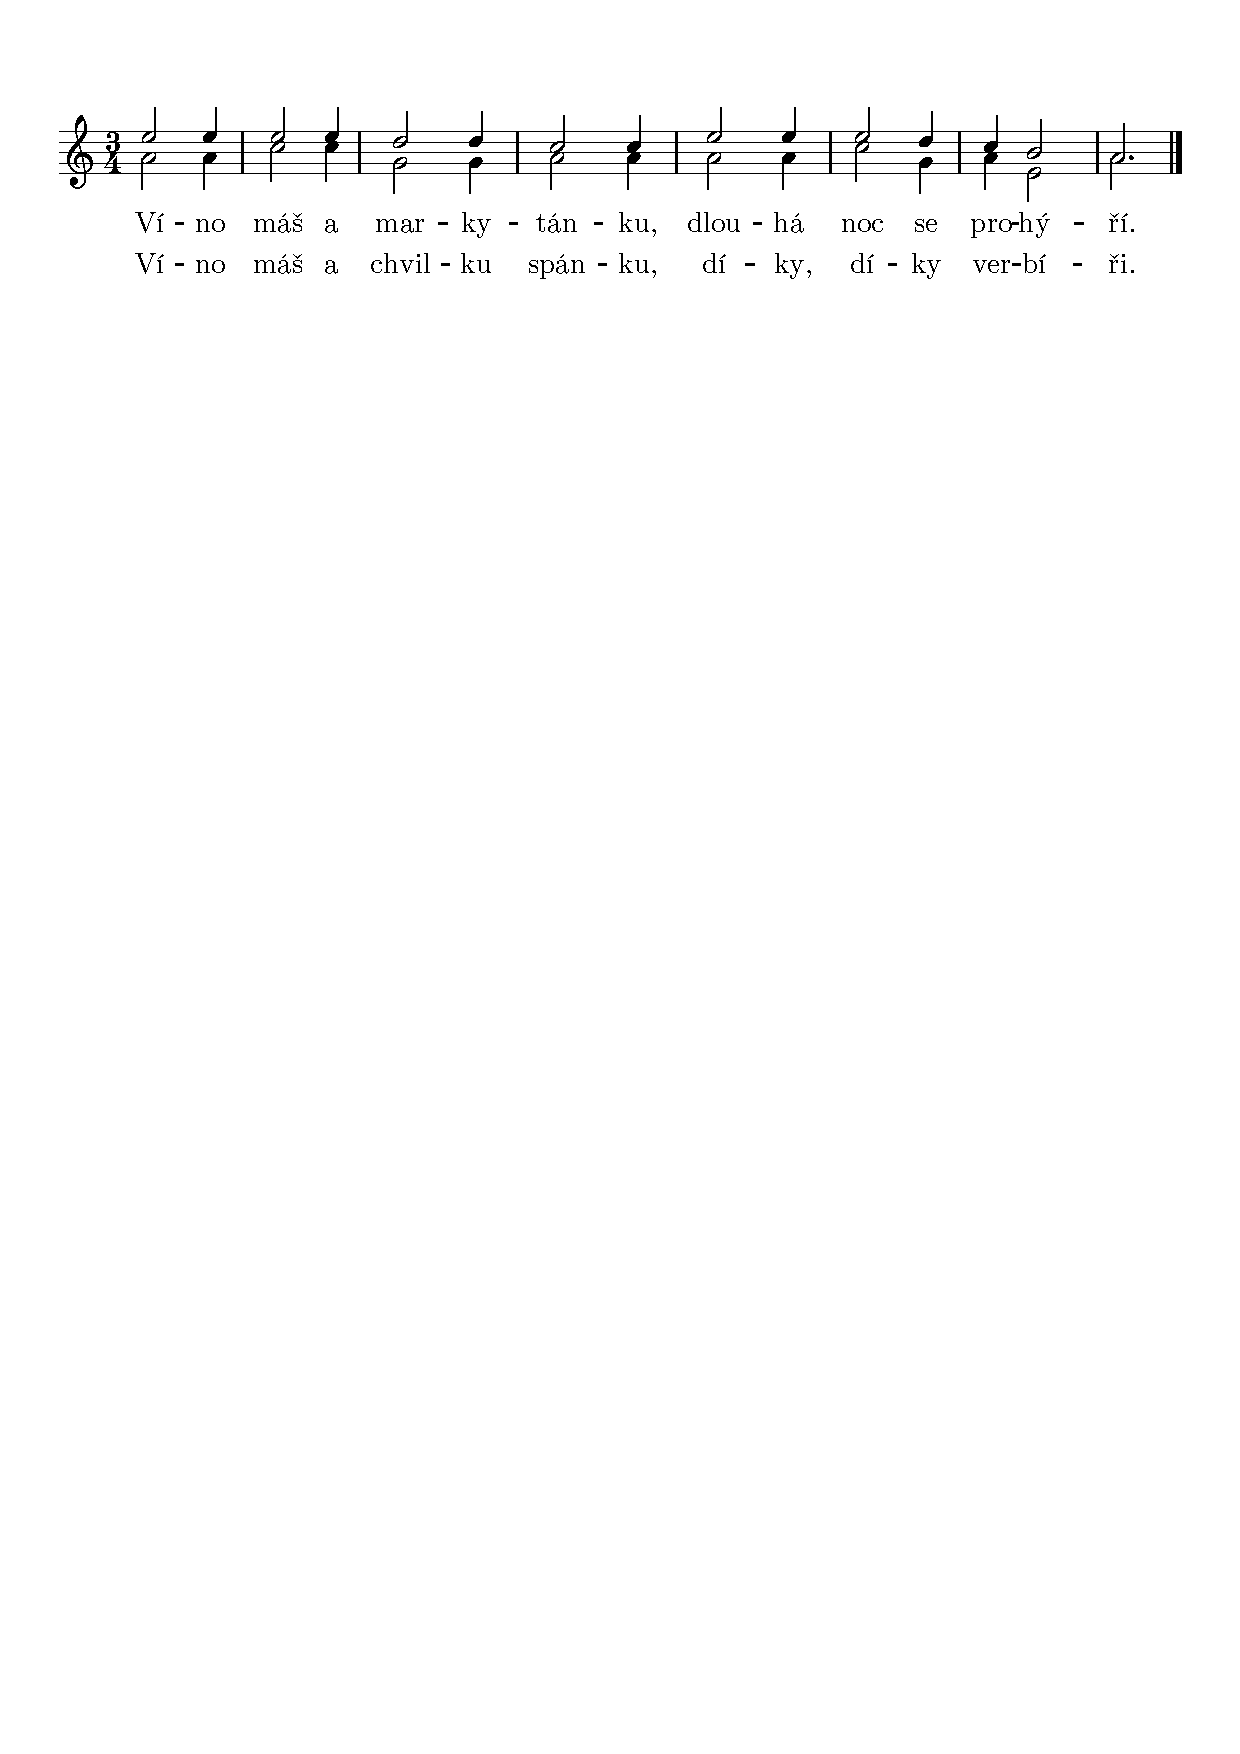
\includegraphics[width=\linewidth]{scores/batalion.pdf}

\vers{1}{
\chord{Am}Dříve, než se rozední, kapitán \chord{C}k osedlání \chord{G}rozkaz \chord{Am}\sm dá\sm\chord{Em}vá,\\
\vinv
\chord{Am}ostruhami do slabin ko\chord{G}ně \chord{Am}\sm po\sm\chord{Em}\sm há\sm\chord{Am}ní.\\
Tam na straně polední čekají ženy, zlaťáky a sláva,\\
do výstřelů karabin zvon už vyzvání.
}

\refrain{
\chord{Am}Víno na ku\chord{C}ráž a \chord{G}pomilovat marky\chord{Am}tánku,\\
\vinv
zítra do Bur\chord{C}gund bata\chord{G}lion \chord{Am}\sm za\sm\chord{Em}\sm mí\sm\chord{Am}ří.\\
Víno na kuráž a k ránu dvě hodinky spánku,\\
díky, díky vám královští verbíři.
}

\vers{2}{
Rozprášen je batalion, poslední vojáci se k zemi hroutí,\\
na polštáři z kopretin budou věčně spát.\\
Neplač sladká Marion, verbíři nové chlapce přivedou ti,\\
za královský hermelín padne každý rád.
}\refsm{}
\newpage
